%--------------------------------------------------
%  Clase 8 – Componentes conexas, conjunto de Cantor y compacidad
%--------------------------------------------------
%  (Para compilar la animación se necesita \usepackage{animate})


\subsection{Componentes conexas y arcoconexas}

\paragraph{\textbf{Definición.}}
Sea $A\subseteq X$.  
Decimos que $A$ es una \emph{componente conexa} (resp.\ \emph{arco conexa}) si $A$ es conexo (resp.\ arcoconexo) y es maximal con esa propiedad; es decir, si $B$ es conexo y $A\subseteq B\subseteq X$, entonces $A=B$.

\paragraph{\textbf{Definición.}}
Un espacio $X$ es \emph{totalmente disconexo} si todas sus componentes conexas son puntos.

\paragraph{\textbf{Ejemplos.}}
\begin{itemize}
  \item El espacio $(X,\mathcal T_{\text{discreta}})$ es totalmente disconexo.
  \item El subespacio $\mathbb Q\subseteq\mathbb R$ es totalmente disconexo.
\end{itemize}

\paragraph{\textbf{Demostración.}}
Sea $A\subseteq\mathbb Q$ conexo.  
Supongamos que $|A|>1$ y tomemos $a,b\in A$ con $a<b$.  
Como $A$ es un intervalo, $[a,b]\subseteq A$.  
Existe $\xi\in[a,b]$ tal que $\xi\in\mathbb R\setminus\mathbb Q$, lo que implica
\[
\xi\in\mathbb Q\cap(\mathbb R\setminus\mathbb Q),
\]
contradicción.

\paragraph{\textbf{Nota.}}
En $\mathbb R$, arco conexo equivale a ser un intervalo; en particular, arco conexo implica conexo.

\paragraph{\textbf{Pregunta.}}
¿Existe un subespacio de $\mathbb R$ que sea
\begin{itemize}
  \item totalmente disconexo,
  \item cerrado,
  \item y sin puntos aislados?
\end{itemize}
Sí: el \emph{conjunto de Cantor}.

\paragraph{Nota:} Un \emph{punto aislado} de $A$ es un $x\in A$ para el cual existe un entorno $U$ con $U\cap A=\{x\}$.

\paragraph{Nota:} Espacios discretos y subespacios densos numerables son totalmente disconexos.

\subsubsection{El conjunto de Cantor}

%--------------------------------------------------
%  Animación de la construcción del conjunto de Cantor
%--------------------------------------------------
%
%  Nota: requiere los paquetes   \usepackage{tikz,animate}
%        (la mayoría del curso ya usa tikz; basta añadir animate).
%
Definimos una sucesión de conjuntos cerrados $(C_n)_{n\ge0}$ por
\begin{align*}
C_0 &\subseteq C_1 \subseteq C_2 \subseteq \dotsb \subseteq C_n \subseteq \dotsb
\end{align*}
% --- Animación de Cantor en niveles (lienzo fijo) ---
% Requiere: \usepackage{tikz,animate}

% --- Animación de Cantor por niveles con resaltado de eliminación ---
\begin{center}
    \begin{animateinline}[poster=first,controls,loop]{2} % 2 fps

  %------------------ C_0 ------------------
  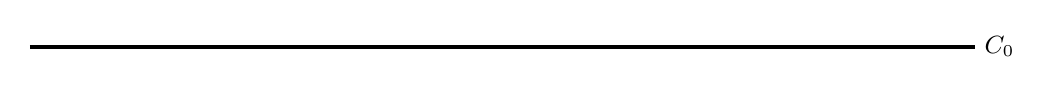
\begin{tikzpicture}[x=12cm,y=1cm]
    \draw[ultra thick] (0,0) -- (1,0);
    \node[right] at (1,0) {\small $C_0$};
  \end{tikzpicture}
  \newframe

  %------------------ C_1 ------------------
  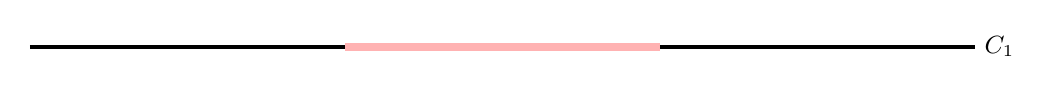
\begin{tikzpicture}[x=12cm,y=1cm]
    % estado anterior (gris)
    \draw[line width=0.6pt,gray] (0,0) -- (1,0);
    % tercio que se elimina
    \fill[red!30] (1/3,0.05) rectangle (2/3,-0.05);
    % Cantor tras la eliminación
    \draw[ultra thick] (0,0) -- (1/3,0);
    \draw[ultra thick] (2/3,0) -- (1,0);
    \node[right] at (1,0) {\small $C_1$};
  \end{tikzpicture}
  \newframe

  %------------------ C_2 ------------------
  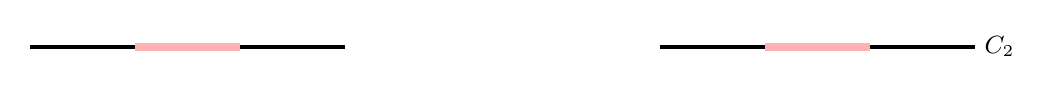
\begin{tikzpicture}[x=12cm,y=1cm]
    % estado anterior en gris
    \draw[line width=0.6pt,gray] (0,0) -- (1/3,0);
    \draw[line width=0.6pt,gray] (2/3,0) -- (1,0);
    % tercios eliminados
    \fill[red!30] (1/9,0.05) rectangle (2/9,-0.05);
    \fill[red!30] (7/9,0.05) rectangle (8/9,-0.05);
    % C_2 resultante
    \foreach \a in {0,2,6,8} {
      \draw[ultra thick] (\a/9,0) -- ++(1/9,0);
    }
    \node[right] at (1,0) {\small $C_2$};
  \end{tikzpicture}
  \newframe

  %------------------ C_3 ------------------
  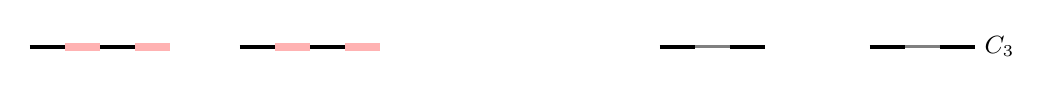
\begin{tikzpicture}[x=12cm,y=1cm]
    % estado anterior en gris
    \foreach \a in {0,2,6,8} {
      \draw[line width=1pt,gray] (\a/9,0) -- ++(1/9,0);
    }
    % tercios eliminados
    \foreach \a in {0,2,6,8} {
      \fill[red!30] (\a/27+1/27,0.05) rectangle (\a/27+2/27,-0.05);
    }
    % C_3 resultante
    \foreach \a in {0,2,6,8,18,20,24,26} {
      \draw[ultra thick] (\a/27,0) -- ++(1/27,0);
    }
    \node[right] at (1,0) {\small $C_3$};
  \end{tikzpicture}
  \newframe

  %------------------ C_4 ------------------
  \begin{tikzpicture}[x=12cm,y=1cm]
    % estado anterior en gris
    \foreach \a in {0,2,6,8,18,20,24,26} {
      \draw[line width=1pt,gray] (\a/27,0) -- ++(1/27,0);
    }
    % tercios eliminados
    \foreach \a in {0,2,6,8,18,20,24,26} {
      \fill[red!30] (\a/81+1/81,0.05) rectangle (\a/81+2/81,-0.05);
    }
    % C_4 resultante
    \foreach \a in {0,2,6,8,18,20,24,26,54,56,60,62,72,74,78,80} {
      \draw[ultra thick] (\a/81,0) -- ++(1/81,0);
    }
    \node[right] at (1,0) {\small $C_4$};
    \end{tikzpicture}

    \end{animateinline}
\end{center}

\begin{align*}
C_0 &= [0,1],\\
C_1 &= [0,1]\setminus\!\left(\tfrac13,\tfrac23\right),\\
C_2 &= C_1\setminus\!\Bigl[\!\left(\tfrac19,\tfrac29\right)\cup\left(\tfrac79,\tfrac89\right)\Bigr],\\
\vdots\\
C_n &= C_{n-1}\setminus\bigcup_{k=1}^{3^{\,n-1}-1}\!
       \left(\tfrac{1+3k}{3^{\,n}},\tfrac{2+3k}{3^{\,n}}\right).
\end{align*}


Cada $C_n$ se obtiene de $C_{n-1}$ eliminando el tercio abierto central de cada intervalo de $C_{n-1}$.
\begin{itemize}
  \item $C_n$ es cerrado.
  \item $C_n$ tiene $2^{n}$ componentes conexas, cada una de longitud $\frac{1}{3^{n}}$.
  \item $C_n$ es la unión de $2^{n}$ intervalos cerrados de longitud $\frac{1}{3^{n}}$.
\end{itemize}

Definimos el \emph{conjunto de Cantor}
\begin{align*}
\mathcal C=\bigcap_{n=0}^{\infty} C_n.
\end{align*}

% \begin{center}
% 
\includegraphics[width=.8\linewidth]{image-5.png}
% \end{center}

\paragraph{\textbf{Propiedades.}}
\begin{enumerate}
  \item $\mathcal C$ es compacto y perfecto.
  \item $\mathcal C$ es totalmente disconexo.
  \item $\mathcal C$ no contiene puntos aislados. 
\end{enumerate}
$\le\frac{1}{3^{n}}$.

\paragraph{\textbf{Demostración.}}
\begin{enumerate}
  \item $\mathcal C$ es compacto porque es la intersección de una sucesión de conjuntos compactos.
  \item Para demostrar que $\mathcal C$ no contiene intervalos, supongamos que existen $\epsilon>0$ y $x\in\mathcal C$ tales que $(x-\epsilon,x+\epsilon)\subseteq\mathcal C$.  
  Como $\mathcal C\subseteq C_n$ para todo $n$, dicha inclusión forzaría
  \[
  (x-\epsilon,x+\epsilon)\subseteq C_n,
  \]
  lo cual es imposible porque los intervalos de $C_n$ tienen longitud $\le\frac{1}{3^{n}}$.
  \item
   Sea $x\in\mathcal C$. Para todo $n$, $x\in C_n$, pero $C_n$ es union de intervalos cerrados, sea  $I_n$ el intervalo de $C_n$ que contiene a $x$. Si $m>n$ $I_m\subseteq I_n$:

  % Para cada $n$, $x$ pertenece a un intervalo cerrado $I_n\subseteq C_n$ con
  % \[
  % \operatorname{diam}(I_n)=\frac{1}{3^{n}},\qquad
  % I_{n+1}\subseteq I_n.
  % \]
  % Entonces
  % \[
  % \bigcap_{n=0}^{\infty} I_n=\{x\}.
  % \]
  % Dado $\epsilon>0$, elija $n$ con $\frac{1}{3^{n}}<\epsilon$; entonces $I_n\subseteq(x-\epsilon,x+\epsilon)$,  puesto que los limites de $I_n$ están en a lo mas una distancia de $\frac{1}{3^{n}}$ de $x$.
  % \[
  % (x-\epsilon,x+\epsilon)\cap\mathcal C\supseteq I_n\neq\{x\},
  % \]
  % de modo que $x$ no es aislado.

  % Sea $x\ in \mathcal C$.
\begin{align*}
\operatorname{diam}(I_n) = \frac{1}{3^n} 
% \to 0 \quad \text{cuando } n \to \infty
\end{align*}
y
\begin{align*}
\bigcap_{n=0}^{\infty} I_n = \{x\}
\end{align*}
Sea $\epsilon > 0$, veamos que $(x-\epsilon, x+\epsilon) \cap \mathcal C \neq \{x\}$.  Sea $I_n$ tal que $\frac{1}{3^n} < \epsilon$, luego $I_n \subseteq (x-\epsilon, x+\epsilon)$. Por que los limites de $I_n = [a_n,b_n]$ estarán una distancia a los mas $\frac{1}{3^n}$ de $x$, luego tenemos los siguientes casos:
\begin{center}
  %--------------------------------------------------
  % Caso 1 : |x - a_n| ≤ |x - b_n|
  %--------------------------------------------------
  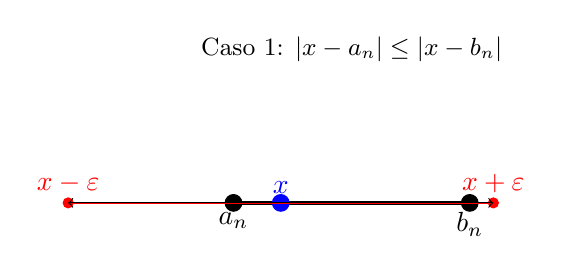
\begin{tikzpicture}[scale=3]
    \node at (0.5,0.65) {\small Caso 1: $|x - a_n| \le |x - b_n|$};
    
    % Intervalo I_n = [a_n,b_n]
    \draw[ultra thick] (0,0) -- (1,0);
    \filldraw (0,0) circle (1pt) node[below] {$a_n$};
    \filldraw (1,0) circle (1pt) node[below] {$b_n$};

    % Punto x
    \coordinate (x1) at (0.2,0);
    \draw[blue,fill=blue] (x1) circle (1pt) node[above] {$x$};

    % Intervalo abierto (x-ε,x+ε) que contiene [a_n,b_n]
    \def\epslen{0.9}             % longitud ε a cada lado de x
    \coordinate (L1) at ([xshift=-\epslen cm]x1);
    \coordinate (R1) at ([xshift=\epslen cm]x1);

    % Segmento rojo
    \draw[red,line width=1pt] (L1) -- (R1);
    % Extremos abiertos y rotulados
    \draw[red,fill=red] (L1) circle (0.6pt) node[above] {$x-\varepsilon$};
    \draw[red,fill=red] (R1) circle (0.6pt) node[above] {$x+\varepsilon$};

    % Flecha que indica 2ε
    \draw[<->] (L1) -- (R1);
  \end{tikzpicture}
  \hspace{1cm}
  %--------------------------------------------------
  % Caso 2 : |x - b_n| < |x - a_n|
  %--------------------------------------------------
  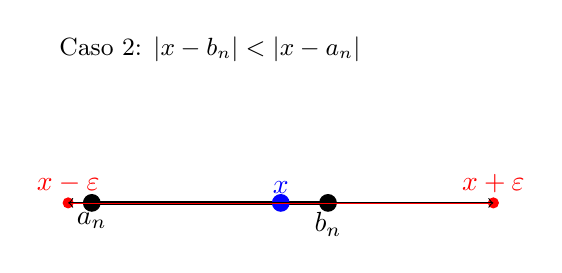
\begin{tikzpicture}[scale=3]
    \node at (0.5,0.65) {\small Caso 2: $|x - b_n| < |x - a_n|$};
    
    % Intervalo I_n = [a_n,b_n]
    \draw[ultra thick] (0,0) -- (1,0);
    \filldraw (0,0) circle (1pt) node[below] {$a_n$};
    \filldraw (1,0) circle (1pt) node[below] {$b_n$};

    % Punto x
    \coordinate (x2) at (0.8,0);
    \draw[blue,fill=blue] (x2) circle (1pt) node[above] {$x$};

    % Intervalo abierto (x-ε,x+ε) que contiene [a_n,b_n]
    \def\epslen{0.9}
    \coordinate (L2) at ([xshift=-\epslen cm]x2);
    \coordinate (R2) at ([xshift=\epslen cm]x2);

    \draw[red,line width=1pt] (L2) -- (R2);
    \draw[red,fill=red] (L2) circle (0.6pt) node[above] {$x-\varepsilon$};
    \draw[red,fill=red] (R2) circle (0.6pt) node[above] {$x+\varepsilon$};

    \draw[<->] (L2) -- (R2);
  \end{tikzpicture}
\end{center}
\begin{align*}
|x-a_n| \leq \frac{1}{3^n} < \epsilon \quad \Rightarrow a_n \in (x-\epsilon,x+\epsilon)\\
|x -b_n| \leq \frac{1}{3^n} < \epsilon \quad \Rightarrow b_n \in (x-\epsilon,x+\epsilon)\\
\end{align*}

entonces $a_n \in (x-\epsilon, x+\epsilon)$. 
Luego $I_n \subseteq (x-\epsilon, x+\epsilon)$ Entonces $a_n \in \mathcal C$ por los limites de cualquier intervalo de $C_n$ estan en $\mathcal C$.Luego:
\begin{align*}
a_n \in (x-\epsilon, x+\epsilon) \cap \mathcal C \\
b_n \in (x-\epsilon, x+\epsilon) \cap \mathcal C
\end{align*}
Asi que $x$ no es aislado.
\end{enumerate}
\paragraph{\textbf{Ejercicios.}}

Consulte Hatcher, págs.\,25–26, ejercicios 8 y 9.  
Consulte Viro–Ivanov, pág.\,15. [2'12x]

\subsection{Compacidad}

\paragraph{\textbf{Definición.}}
Un espacio topológico $X$ es \emph{compacto} si para toda familia de abiertos $\{U_i\}_{i\in I}$ que cubre $X$,
\begin{align*}
X=\bigcup_{i\in I}U_i,
\end{align*}
existe una subfamilia finita $\{U_{i_1},\dots,U_{i_n}\}$ tal que
\begin{align*}
X=\bigcup_{j=1}^{n}U_{i_j}.
\end{align*}

%--------------------------------------------------
%  Fin de la clase 8
%--------------------------------------------------